\documentclass[a4paper,14pt,onecolumn]{article}


\usepackage[dvips]{graphics}
\usepackage{color}
\usepackage{epsfig}
\usepackage{amsmath}
\usepackage{graphicx}
\bibliographystyle{ieeetr}

\setlength{\textwidth}{6.27in}
\setlength{\textheight}{9.69in}
\setlength{\topmargin}{0.0in}
\setlength{\oddsidemargin}{0.0in}			% Customisable
\setlength{\headheight}{0.0in}
\setlength{\headsep}{0.0in}
\setlength{\topskip}{0.0in}

\fontencoding{T1}		% Font specification : Times New Roman, Bold, Normal, 18
\fontfamily{cmr}		% Roman
\fontseries{m}			% Medium
\fontshape{n}			% Upright
\fontsize{14pt}{5}		
\linespread{1.5}		% Vertical spacing between lines
\selectfont			% Select the specified font

\begin{document}
\pagestyle{empty}
%_____________________________________________________________________________________________ 
% Title page: Specifies a custom-made title page
%_____________________________________________________________________________________________ 
\DeclareGraphicsExtensions{.png, .ps}
\begin{titlepage}
\begin{center}
\Large{\bf{A PROJECT REPORT\\}}		% Large = 14.40
\Large{\bf{ON\\}}		% Large = 14.40
\begin{center}\color{blue}
\LARGE{\bf{ ``MINING CLASSIFICATION RULES FROM DATABASE USING ARTIFICIAL NEURAL NETWORK''\\}}	% LARGE = 17.28
\end{center}
\Large{Under the guidance of\\ }\begin{center}\color{red}
\Large{\bf{HOD Prof. Mrs. S. Shinde}\\}\end{center}
\vspace{8pt}
\Large{\em{Submitted by\\}}
\begin{table}[htbp]
	\begin{center}
    \color{red}
	\begin{tabular}{ l c c l }
	\Large{B8338503} & & & \Large{Prashant  P. Avaghade} \\ 
	\Large{B8338513} & & & \Large{Datta G. Diware} \\
	\Large{B8338528} & & & \Large{Mahesh S. kshatriya} \\
	\Large{B8338559} & & & \Large{Nikhilesh S. Shinde} \\
      \Large{B8338570} & & & \Large{Sumit S.Wankhede} \\
	\end{tabular}
	\end{center}
	\end{table}
%names of advisors
\Large{\em{Towards the Partial fulfillment of
Final year degree course in\\B.E. Information Technology\\
Of\\University of Pune
In the academic year
2011-12
\\}}
\vspace{3pt}
\vspace{10pt}
%pccoe logo added
\begin{figure}[h]
\centering

\includegraphics[width=3cm,height=3cm]{pccoelogo.jpg}
\end{figure}
\Large{\bf{DEPARTMENT OF INFORMATION TECHNOLOGY,\\ 
PIMPRI CHINCHWAD COLLEGE OF ENGINEERING, PUNE-46}}
\vfill
\large\bf{(2011-2012)}
\end{center}
\end{titlepage}

\thispagestyle{empty}
\begin{titlepage}
\begin{center}
\Large{\bf{PIMPRI CHINCHWAD EDUCATION TRUST’S
PIMPRI CHINCHWADCOLLEGE OF ENGINEERING
AKURDI, PUNE-411044
\\}}
\end{center}
\begin{center}
\color{red}\Huge{\bf{CERTIFICATE\\}}	
\end{center}
\begin{center}
\bf{
This is to certify that\\
Project work\\
ON}
\end{center}
\begin{center}
\color{blue}\LARGE{\bf{``MINING CLASSIFICATION RULES FROM DATABASE USING ARTIFICIAL NEURAL NETWORK'' \\}}	
\end{center}
\begin{center}
\Large{\em{Submitted by\\}}
\begin{table}[htbp]\color{red}
	\begin{center}
	\begin{tabular}{ l c c l }
	\Large{B8338503} & & & \Large{Prashant  P. Avaghade} \\ 
	\Large{B8338513} & & & \Large{Datta G. Diware} \\
	\Large{B8338528} & & & \Large{Mahesh S. kshatriya} \\
	\Large{B8338559} & & & \Large{Nikhilesh S. Shinde} \\
      \Large{B8338570} & & & \Large{Sumit S.Wankhede} \\
	\end{tabular}
	\end{center}
	\end{table}
%names of advisors


\Large{Under the guidance of\\ }\begin{center}
\color{red}\Large{\bf{HOD Prof. Mrs. S. Shinde}\\}\end{center}
\Large{Towards the Partial fulfillment of
Final year degree course in\\B.E. Information Technology
Of\\University of Pune
In the academic year
2011-12
\\}
\vspace{3pt}

% Horizontal spacing used to keep the signatures in columns at the ends of lines

%SIGNATURE\hspace{\stretch{1}}SIGNATURE\\
	\begin{table}[htbp]
	\begin{center}
	\begin{tabular}{ l c c c c l }
	\bf{Prof. S. V. Shinde} & \bf{Prof. R. G. Pise} & \bf{Prof. S. V.Shinde} & \bf{Prof.A.M.Fulambarkar}\\[0.3cm] 
	\bf{Project Guide} & \bf{Project Coordinator} & \bf{HoD} & \bf{Principal}\\
	\end{tabular}
	\end{center}
	\end{table} 
\end{center}
\end{titlepage}
\begin{titlepage}
\begin{center}
\huge{\bf{ACKNOWLEDGEMENT\\}}\end{center}
\large{
\begin{sloppypar}
Any accomplishment requires converted efforts of many people and this project is no different. We are highly obliged and grateful to all those who have helped us in the development of this Project and provided all encouragement that has helped us immensely in our project work.
\end{sloppypar}
\begin{sloppypar}
It is our pleasure to present the project entitled \textbf{``MINING CLASSIFICATION RULES FROM DATABASE USING ARTIFICIAL NEURAL NETWORK''} which has been a throughout joint effort. Since the time we have started working on this project, we have thoroughly been engrossed with the technological exploration of the field. We acquired knowledge by reading different books and searching on the Internet.
\end{sloppypar}\begin{sloppypar}
 We take this opportunity to thank our respected \textbf{Project Guide Prof.Swati V. Shinde} without whose constant support, help and encouragement, this endeavor of ours wouldn’t have materialized.
\end{sloppypar}
\begin{sloppypar}
We thank our Principal \textbf{Dr.A.M.Fulambarkar} Project coordinator \textbf{Prof.R.G.Pise} and HOD \textbf{Prof.S.V.Shinde} for creating a wonderful learning environment. Finally, we thank all teaching and non-teaching staff who has associated directly/indirectly in the execution of this project work.
\end{sloppypar}
\begin{sloppypar}
Last but not least, we are also grateful to our friends for their valuable suggestions.\\
\end{sloppypar}}
\begin{table}[hbp]
 \begin{center}
    \begin{tabular}{   p{9cm}  l  l  }

                      \,               &    B8338503 & Prashant  P. Avaghade \\  
                       \,               &   B8338513 & Datta G. Diware \\  
                      \,                 &  B8338528 & Mahesh S. kshatriya \\  
                        \,             &    B8338559  & Nikhilesh S. Shinde \\  
                        \,             &    B8338570  & Sumit S.Wankhede \\  

    \end{tabular}
\end{center}
\end{table} 
\end{titlepage}
\begin{titlepage}
\begin{center}
\huge{\bf{ABSTRACT\\}}\end{center}
\large{
The important task in data mining is the classification of the data into the predefined groups or classes. One of the commonly used classifier technique is Artificial Neural Networks (ANN) [1]. Although ANN usually reaches high classification accuracy, the obtained results sometimes may be incomprehensible [2]. Due to this fact various methods have been proposed to extract the rules from ANN which justifies the classification results given by ANN. For this the trained neural network is pruned for removing the inputs that are not needed for solving the problem. The pruned network serves to filter noise that might be present in the data [2]. The proposed research work shall be based on extracting optimized the rules from ANN which justifies the classification results given by ANN.}
\end{titlepage}

\pagenumbering{roman}		% Lowercase roman numbering for prelim sections


\newpage
\thispagestyle{empty}
\tableofcontents		% *Generate* the table of contents. No content - no table
				% LATEX needs to run 2-3 times over source to get this correct

\newpage
\listoftables


\newpage
\listoffigures

\newpage
\pagenumbering{arabic} % Change to Arabic numbers for main chapters.
\section{INTRODUCTION}
 Neural Networks are successful in acquiring hidden knowledge in datasets. Their biggest weakness is that the knowledge they acquire is represented in a form not understandable to humans. Researchers tried to address this problem by extracting rules from trained Neural Networks. Most of the proposed rule extraction methods required specialized type of Neural Networks; some required binary inputs and some were computationally Lack of explanation capability is one of the most important reasons why Neural Networks do not get the necessary interest in some parts of the industry.\\
          In most of the real world applications (especially in safety critical applications) users want to know the reasoning behind the conclusion of a learning system or an expert system. Extracting If-Then rules is usually accepted as the best way of extracting the knowledge represented in the Neural Network. Rules extracted from the trained net can be used for explaining the reasoning behind the output of the system. They can also be used in other systems, like expert systems or in systems for discovering previously unknown features in the data (data mining).\\ 
          Generalization of the system can also be improved by having a better feature representation. Quality of the rules can be measured by Accuracy, Fidelity, and Comprehensibility. Fidelity is the fraction of instances on which Neural Network and the extracted rules give the same output. Comprehensibility is measured by the size of the rule set and by the number of antecedents in each rule.

\subsection{Basic Concepts}

\subsubsection{ Data Mining}
                       Data mining (DM), also known as ‘‘knowledge discovery in databases” (KDD), is the process of discovering meaningful patterns in huge databases [3]. In addition, it is also an application that can provide significant competitive advantages for making the right decision.  DM is an explorative and complicated process involving multiple iterative steps.

\subsubsection{Data Mining Tasks}
  \begin{itemize}
\item Classification              : Classifies a data item into one of several predefined categories.

\item Regression                 : Maps a data item to a real-valued prediction variable.

\item Clustering                  : Maps a data item into a cluster, where clusters are natural groupings of data items based on similarity metrics.

\item Association rules        : Describes association relationship among different attributes.

\item Summarization           : Provides a compact description for a subset of data.

\item Dependency modeling : Describes significant dependencies among variables.

\item Sequence analysis       : Models sequential patterns, like time-series analysis. The goal  is to model the state of the process generating the sequence or to extract and  report deviations and trends over time.
\end{itemize}

 \subsubsection{Classification Techniques} \begin{itemize}
\item Decision Tree based Methods
\item Rule-based Methods
\item Memory based reasoning
\item Genetic Algorithms
\item Support Vector Machines
\item Neural Networks 
\end{itemize}

\subsubsection{Classification }
Learn a method for predicting the instance class from pre-labeled (classified) t  Instances.

\begin{figure}[h]
\begin{center}
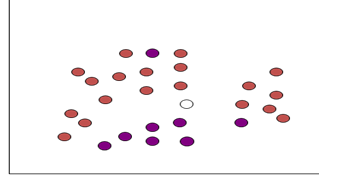
\includegraphics[height=1in,width=2in]
{classficationGraph.jpg}  
\caption{Classification Graph}
\end{center}
\end{figure} 

\subsubsection{Decision Trees  }
            An internal node is a test on an attribute. A branch represents an outcome of the test, e.g. Color=red. A leaf node represents a class label or class label distribution. At each node, one attribute is chosen to split training examples into distinct classes as much as possible A new instance is classified by following a matching path to a leaf node.

\begin{figure}
\begin{center}
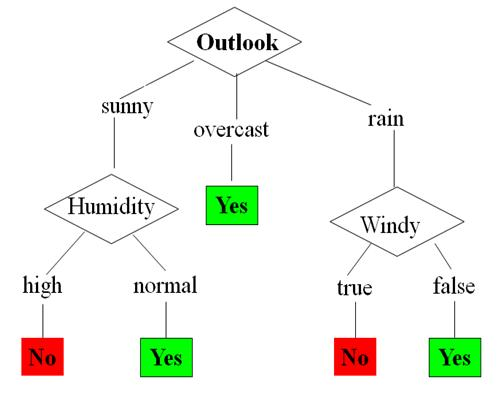
\includegraphics[height=2in,width=2.5in]
{decisiontree.jpg}  
\caption{Example Tree for “Play?”}
\end{center}
\end{figure} 

\subsubsection{Neural Network}
\begin{enumerate}
\item What is Neural Network?\\
              A neural network is a powerful data modeling tool that is able to capture and represent complex input/output relationships. It is a biologically motivated approach to machine learning.


Neural networks resemble the human brain in the following two ways: 
 \begin{itemize}	
\item A neural network acquires knowledge through learning. 
\item A neural network's knowledge is stored within inter-neuron connection strengths known as synaptic weights.
\end{itemize}

\begin{figure}[hbp]
\begin{center}
\includegraphics[height=2in,width=2in]
{Neuron.jpg}  
\caption{Biological Neuron}
\end{center}
\end{figure}  

\begin{figure}[hbp]
\begin{center}
\includegraphics[height=3in,width=4in]
{Neuralnetwork.jpg}  
\caption{Basic Architecture of Neural Network}
\end{center}
\end{figure} 

\item Back propagation and Feed-Forward NN\\
       It is a supervised learning method, and is a generalization of the delta rule. It requires a teacher that knows, or can calculate, the desired output for any input in the training set. It is most useful for feed-forward networks (networks that have no feedback, or simply, that have no connections that loop). The term is an abbreviation for "backward propagation of errors". Back propagation requires that the activation function used by the artificial neurons (or "nodes") be differentiable

\begin{figure}[hbp]
\begin{center}
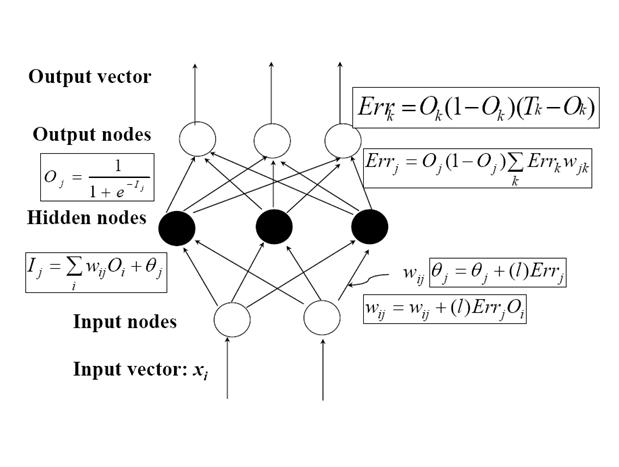
\includegraphics[height=4in,width=4in]
{BBNeuralnetwork.jpg}  
\caption{Backproagation Neural Network}
\end{center}
\end{figure} 

The ANN is composed of richly interconnected non-linear nodes that do processing in parallel. The connection weights are modifiable, allowing ANN to learn directly from examples without requiring or providing an analytical solution to the problem. The most popular forms of learning are:

\begin{itemize}

\item Supervised learning: Patterns for which both their inputs and outputs are known are presented to the ANN. The task of the supervised learner is to predict the value of the function for any valid input object after having seen a number of training examples. ANN employing supervised learning has been widely utilized for the solution of function approximation and classification problems.  

\item Unsupervised learning: Patterns are presented to the ANN in the form of feature values. It is distinguished from supervised learning by the fact that there is no a priori output. ANN employing unsupervised learning has been successfully employed for data mining and classification tasks. The self-organizing map (SOM) and adaptive resonance theory (ART) constitutes the most popular examples of this class. A backpropagation network (BPN) is a neural network that uses a supervised learning method and feed-forward architecture. A BPN is one of the most frequently utilized neural network techniques for classification and prediction and is considered an advanced multiple regression analysis that can accommodate complex and non-linear data relationships.
\end{itemize}

\item Neural Network and data mining
\begin{figure}[hbp]
\begin{center}
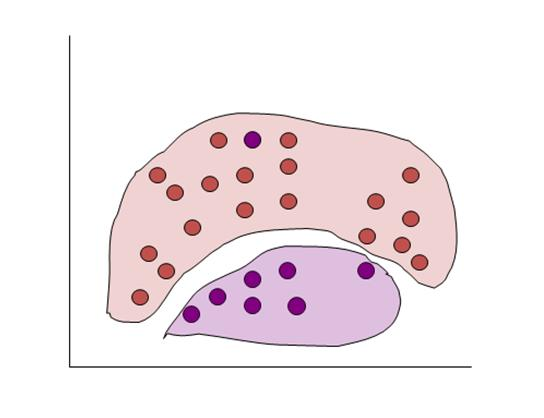
\includegraphics[height=3in,width=3in]
{NNdatamining.jpg}  
\caption{Neural Network in Data Mining}
\end{center}
\end{figure}
\begin{itemize}
\item Can select more complex regions.
\item Can be more accurate.
\item Also can overfit the data – find patterns in random noise.
\end{itemize}
\end{enumerate}

\subsubsection{Application}

\begin{itemize}
\item Key finance decision making problem e.g. credit card approval.
\item Medical Application e.g. cancer patient classification depending upon symptoms attributes.
\item Pattern Recognition.
\item Image Processing.
\end{itemize}

\newpage
\section{Literature Survey}
          To reveal the information concealed in an ANN, researchers have proposed a number of rule extraction techniques. One of the first rule extraction techniques from neural network was proposed by Galant . He was working on connectionist expert systems. In this work, each ANN node is represented as a conceptual entity.\\
     Yueh-Min Huanga and  Chun-Min Hunga [8] have  addressed the problem of imbalanced class distributions. This paper analyzes different classification algorithms that were employed to predict the creditworthiness of a bank’s customers based on checking account information. A series of experiments were conducted to test the different techniques. The objective is to determine a range of credit scores that could be implemented by a manager for risk management. Also a strategy of data cleaning for handling such a real case with imbalanced distribution data is presented by them.\\
      Wei-Sen Chen  and Yin-Kuan Du  have used the artificial neural network (ANN) and data mining (DM) techniques to construct the financial distress prediction model . In this paper traditional Data Mining- Clustering approach is compared with ANN approach. After this experimentation authors have stated that the ANN approach obtains better prediction accuracy than the DM clustering approach. Therefore, the authors have concluded that the artificial intelligent (AI) approach could be a more suitable methodology than traditional statistics for predicting the potential financial distress of a company.\\
      Humar Kahramanli and  Novruz Allahverdi [7] have presented the technique of mining the classification rules for Liver Disorders using adaptive activation function. In this study the authors have first trained the neural network with adaptive activation function. Then the rules are extracted from this trained neural network by using the OptaiNET that is an Artificial Immune Algorithm (AIS).\\
    The used Neuro-Adaptive function is as follows:\\
\begin{center}
$Ø(x) =\frac{A1 e^{- x2}+A2}{(1+e^{-B*x})}$\\
\end{center}

Where, A1, A2 and B are real variables which will be adjusted during training.
     In this paper, for rule extraction the first ANN which classifies the dataset was designed. Then Opt-aiNET algorithm was executed for extraction of rules from this ANN. Finally, the extracted rules were decoded. Produced rules diagnosed correctly 192 samples from 200 belong to Class 0 and 135 samples from 145 belongs to Class1. It means system achieve 96% and 93% correctly diagnosis for Class 0 and Class 1 respectively. In summary the system correctly diagnosed 94.8% of whole samples.\\
     In paper [9] association rules have been composed using Apriori algorithm and transactions, which provide these rules, were eliminated. This provides shrinking database. Then ANN has been trained and used Opt-aiNET for composing rule set. It’s been observed that this method increased classification accuracy despite decreasing number of rules.\\ 
     Humar Kahramanli and  Novruz Allahverdi [1] have presented the method that uses Artificial Immune Systems (AIS) algorithm to extract rules from trained hybrid neural network [6]. The datasets used are Cleveland heart disease and Hepatitis data taken from UCI machine learning repository.\\ 
     The performance metrics used in this algorithm are accuracy, sensitivity and specificity which are the common performance metrics used in medical diagnosis tasks. The measure of the ability of the classifier to produce accurate diagnosis is determined by accuracy. The measure of the ability of the model to identify the occurrence of a target class accurately is determined by sensitivity. The measure of the ability of the model to separate the target class is determined by specificity. So that accuracy, sensitivity and specificity are calculated as follows:\\

\begin{center}
$Accuracy=\frac{Total number  of  correctly diagnosed cases}{Total number of cases}$\\[4mm]

$Sensitivity=\frac{Total number of positive cases correctly diagnosed}{Total number of positive cases }$\\[4mm]

$Specificity=\frac{Total number of negative cases correctly diagnosed T}{Total number of negative cases}$\\[4mm]
\end{center}
     This method achieves accuracy values of 96.4% and 96.8% for Cleveland heart disease dataset and Hepatitis dataset respectively.\\
     Miguel Rocha and Paulo Cortez [10] have presented the use of Evolutionary Computation (EC) as a promising alternative for ANN optimization. In this paper two hybrid EC/ANN algorithms are presented: the first evolves neural topologies while the latter performs simultaneous optimization of architectures and weights. Sixteen real-world tasks were used to test these strategies. \\
      Richi Nayak [11] has given a novel methodology “Gyan” that represents the knowledge of a trained network in the form of restricted first-order predicate rules. \\
      In paper [5] the mathematical properties of several error functions with a focus on MLP data classification are analyzed. This analysis led us to propose two parameterized error functions for MLP training. The first one, ESMF, is a monotonic error function applicable only to two-class problems and was shown to perform equally well as other functions. However, it should be extended to the general multi-class problem for a better evaluation of its capability. The second one, EExp, an exponential-type error function, this function is able to emulate the behaviors of classic error functions and, as a matter of fact, by single parameter adjustment it is able to implement an infinite family of error functions, with different behavior of the error gradient weighting.\\
       By Ajit Narayanan, Edward Keedwell and Dragan Savic [12] have presented a novel approach using genetic algorithms to search for symbolic rules in a trained neural network.       Many rule extraction algorithms have been designed to generate classification rules from NNs that have been trained to distinguish data samples from different classes. These algorithms frequently assume that the input data attributes are discrete in order to make the rule extraction process more manageable. NeuroRule [14] is one such algorithm. A component of NeuroRule is an automatic rule generation method called rule generation (RG). Each rule is generated by RG such that it covers as many samples from the same class as possible with the minimum number of attributes in the rule condition. RG is applied to generate rules that explain the network’s output in terms of the discretized hidden unit activation values and rules that explain the discretized activation values in terms of the discretized attributes of the input data.\\
       Rule eXtraction (RX) [15] is another NN rule extraction algorithm that works on discrete data. RX recursively generates rules by analyzing the discretized hidden unit activations of a pruned network with one hidden layer. When the number of input connections to a hidden unit is larger than a certain threshold, a new NN is created and trained with the discretized activation values as the target output. \\
     The generalized analytic rule extraction (GLARE) algorithm [16] does not require network pruning. It does, however, require that the continuous attributes be first converted to nominal, and then to binary attributes before the algorithm can be applied. While the algorithm is shown to work well on discrete data sets, it does not perform as well as decision tree methods on data sets with continuous attributes. \\
     The orthogonal search-based rule extraction (OSRE) method [17] assumes that the data has been 1-from-N encoded; hence its application is also limited to data with only nominal or ordinal attributes. \\
    Trepan, an algorithm that was developed by Craven and Shavlik [18] also extracts M-of-N rules from an NN. It treats the NN as an oracle to generate additional data samples. This is an important step in trepan as it grows a decision tree by recursive partitioning. As the tree grows, fewer and fewer training samples are available for deciding if a node should be split further. Additional samples are generated by taking into account the distribution of the existing data samples and their labels are determined by the NN oracle. A node in the tree becomes a leaf node if it has sufficiently a high proportion of samples that belong to one class or if the number of internal nodes in the tree has reached the maximum.\\
    There exist algorithms that generate fuzzy rules from NNs. Nefclass [19] is one such algorithm. It works as a three-layer fuzzy NN. The difference between this type of networks and the standard backpropagation NNs lies in the connection weights which represent fuzzy sets and in the activation functions which act as fuzzy set operators. Nefclass employs a fuzzy variant of the backpropagation algorithm to find the characteristic parameters of the membership functions.\\
    Benitez [20] proposed a method for translating the knowledge embedded in an NN into a fuzzy-rule-based system.\\
    Tsukimoto [21] developed an NN rule extraction algorithm that could be applied to continuous data directly. Instead of linear combinations of the inputs as the rule conditions, the rules are represented as continuous Boolean function of the attributes. The algorithm has been tested only on the Iris data set and the accuracy obtained was not as good as the accuracy of the decision tree method C4.5.\\
    The algorithm full rule extraction (full-RE) [22] is able to extract accurate rules from the Iris data set without the need to binarize or normalize the continuous attributes of the data prior to network training. For each hidden node in the network, full-RE generates an intermediate rule that predicts its output according to the linear combinations of the input attributes. In order to obtain the final set of classification rules that do not involve network weights in their rule conditions, full-RE discretizes the input attributes and then solves a linear programming problem to select the relevant discretization boundary.\\
    A recent rule extraction algorithm that works on discrete and continuous data was proposed by Rabuñal [23]. There is, however, no provision for generating rules with separate rule conditions involving discrete and continuous attributes.\\
     Rudy Setiono and Bart Baesens [2] have presented a recursive algorithm for extracting classification rules (RE-RX) from feedforward neural networks that have been trained on data sets having both discrete and continuous attributes. This algorithm shares some similarities with other existing rule extraction algorithms. It assumes that the trained network has been pruned so that irrelevant and redundant network connections and units have been removed. It also makes use of the decision tree method C4.5 to generate rules with only discrete attributes in their conditions. The novel feature of the proposed recursive algorithm lies in the rule set generated. The rules are hierarchical such that only those rules at the deepest level have rule conditions that involve linear combinations of the continuous attributes, while the conditions of all the other rules involve only the discrete attributes. We believe that such rule conditions would greatly increase the comprehensibility of the rules, and hence greatly pave the way to open the NN “black box” wider.\\

\newpage
\section{System requirement and specification }

\subsection{Project Statement}
 Mining classification rules from database using ANN and optimizing the knowledge generated in terms of classification accuracy.\\

 \subsection{Proposing theme of the project}
Recursive Neural Network Rule Extraction for Data with Mixed attributes By Rudy Setiono,Senior Member, IEEE, Bart Baesens, and Christophe Mues [IEEE Transaction on Neural Networks, Vol. 19 No. 2, February 2008 pp. 299-307]
In this paper, a recursive algorithm for extracting classification rules from feedforward neural networks that have been trained on data sets having both discrete and continuous attributes is presented Real-world classification problems usually involve both discrete and continuous input attributes. For such problems, all the continuous attributes must be discretized if algorithms such as NeuroRule, GLARE, and OSRE are to be used for rule extraction.The drawback of discretizing the continuous attributes is that the accuracy of the networks, and hence the accuracy of the rules extracted from the networks, may decrease. This is because discretization leads to a division of the input space into hyperrectangular regions. Each condition of the extracted rulescorresponds to one of these hyperrectangular regions where all data samples are predicted to belong to one class. Clearly, a data preprocessing step that divides the input space into rectangular subregions may impose unnecessary restrictions on the NNs as classifiers. It is highly likely that the boundaries of the regions that contain data samples from the same class are nonrectangular given that some of the data attributes are continuous.\\

\subsection{Overall Description}
The proposed system presents a justified neural network using rule extraction for classifying pima Indian diabetes patiens.System provides recursively extracted hierarchical rules for describing hidden knowledge of the trained neural network.
A recursive rule extraction algorithm proposed by Rudy Setiono is used for implementing this system

\subsubsection{Overall Steps}
\begin{enumerate}

\item Step 1: (Data collection) The data to be used for classification is collected. 

\item Step 2: (Training and testing data separation) The available data are divided into training and testing data sets of size 80\% and 20\% respectively.

\item Step 3: (Network architecture) network architecture and a learning method are selected. Important considerations are the exact number of perceptrons and the number of layers. 
 
\item Step 4: (Parameter tuning and weight initialization) There are parameters for tuning the network to the desired learning performance level. Part of this step is initialization of the network weights and parameters, followed by modification of the parameters as training performance feedback is received. \\ 
Initialize weight and biases to the random numbers distributed over a small range of values:
 \begin{math}      [{-\alpha \over \sqrt{Ni}} ,{ -\alpha \over \sqrt{Ni}}]\\
                           Where\,N_{i}  -No. \,of \,units\, to \, i^{th}\, unit,\\
				   \alpha  \end{math}   - integer between 1 to 3.       


\begin{figure}[hbp]
\begin{center}
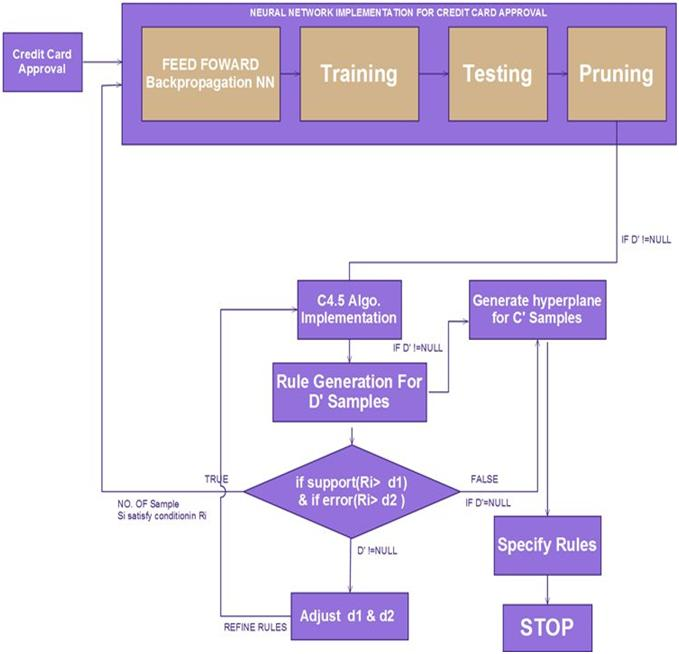
\includegraphics[height=6in,width=6in]{blockdiagram.JPG} 
\caption{ Neural Network Implementation}
\end{center}
\end{figure}


\item Step 5: (Data Normalization) transforms the application data into the type and format required by the ANN. All data must be normalized i.e. all values of the attributes in the database are changed to contain in the interval [0,1] or [-1,1].
Two normalization techniques are used:
\begin{enumerate}
\item Max-Min Normalization.
\item Decimal scaling Normalization. 
\end{enumerate}

\item Step 6: (Training) Training is conducted iteratively by presenting input and desired or output data to the ANN. The ANN computes the outputs and adjusts the weights until the computed outputs are within an acceptable tolerance of the known outputs for the input cases. 

\item Step 7: (Testing) The testing examines the performance of the network using the derived weights by measuring the ability of the network to classify the testing data correctly. 

\item Step 8: (Implementation) Now a stable set of weights are obtained. Now the network can reproduce the desired output for the given inputs like those in the training set. The network is ready to use as a stand-alone system or as part of another software system where new input data will be presented to it and it output will be a recommended decision.  

\end{enumerate}



\newpage
\subsubsection{Pima Indian Diabetes Dataset}
\begin{enumerate}
\item Title: Pima Indians Diabetes Database
\item Sources:
                    Original owners: National Institute of Diabetes and Digestive and
                     Kidney Diseases
\item Past Usage:
 Smith,~J.~W., Everhart,~J.~E., Dickson,~W.~C., Knowler,~W.~C., \&    	            Johannes,~R.~S. (1988). Using the ADAP learning algorithm to forecast
the onset of diabetes mellitus.  In {\it Proceedings of the Symposium   	                               on Computer Applications and Medical Care} (pp. 261--265).  IEEE
                        Computer Society Press.
\item Number of Instances: 768
\item Number of Attributes: 8 plus class 
\item For Each Attribute: (all numeric-valued)
  \begin{enumerate}
  \item Number of times pregnant.
  \item Plasma glucose concentration a 2 hours in an oral glucose tolerance test
  \item Diastolic blood pressure (mm Hg)
  \item Triceps skin fold thickness (mm)
  \item 2-Hour serum insulin (mu U/ml)
  \item Body mass index (weight in kg/  \begin{math}  (height\,in\,m)^{2} \end{math}  )
  \item Diabetes pedigree function
  \item Age (years)
  \item Class variable (0 or 1)
  \end{enumerate}
\item Missing Attribute Values: Yes
\item Class Distribution: (class value 1 is interpreted as ``Tested positive for
   	     diabetes'')
           
    \begin{table}[hbp]
       \begin{center}
            \begin{tabular}{|l|l|}
                     \hline
 					 \multicolumn{2}{|c|}{  Class Value For Number of instances} \\
 					 \hline
 						 0 & 500 \\
 						 1 & 268 \\
                     \hline
           \end{tabular}
        \end{center}
     \caption{Class Distribution}
     \end{table}

\item Brief statistical analysis:
\begin{table}[h!]
 \begin{center}
    \begin{tabular}{ | l | l | l |}
    \hline
    Attribute number & Mean & Deviation  \\ \hline
    1  &	3.8 & 34\\ \hline
    1	&  3.8  &	3-4\\ \hline
	2	& 120.9	 & 32.0\\ \hline
	3	& 69.1 &	19.4\\ \hline
	4	& 20.5	& 16.0\\ \hline
	5	& 79.8	& 115.2\\ \hline
	6	& 32.0	& 7.9\\ \hline
	7	& 0.5	& 0.3\\ \hline
	8	& 33.2 &	11.8\\
    \hline
    \end{tabular}
   \caption{Statistical analysis of the dataset}
\end{center}
\end{table}    
\end{enumerate}
\newpage
\subsubsection{Discrete and continuous attributes}
\begin{itemize}
\item	 \textbf{Discrete Attributes:} Any data measurements that are not quantified on and infinitely divisible numeric scale is called discrete attributes.

\item \textbf{Continuous Attributes:} Any data measurements that are quantified on and infinitely divisible numeric scale is called continues attributes.

\end{itemize}

\subsubsection{Feed forward Neural Network}
\textbf{Neural network training:}\\
Find an optimal weight (W,V).Minimize a function that measures how well the network predicts the desired outputs (class label).
\begin{itemize}
\item Error in prediction for \begin{math} i^{th} sample:
                               e^{i} = {(desired output)^i - (predicted output)^i} \                  
                                         \end{math}
\item Sum of squared error function:\,\begin{math}
                                   E(W,V) = \sum e^i
                                     \end{math}     
\item Cross‐entropy error function:\\ \begin{math}
                           E(W,V) =\- \sum d_i log p_i + (1 - di) log (1 -  p_i)\\\end{math}
  d is the desired output either 0 or 1  \begin{math}d_i \end{math} output, 1 Many optimization methods.          
\item  Gradient descent/error back propagation
\item  Conjugate gradient
\item  Quasi Newton method
\item  Genetic algorithm  
\item  Network is considered well trained if it can predict training data and cross validation data with acceptable accuracy.                                               
\end{itemize}

\subsubsection{Pruning}
Artificial neural networks are considered as efficient computing models and as the universal approximates .The predictive accuracy of neural network is higher than that of other methods or human experts, it is generally difficult to understand how the network arrives at a particular decision due to the complexity of a particular architecture. One of the major criticism is their being black boxes, since no satisfactory explanation of their behavior has been offered. This is because of the complexity of the interconnections between layers and the network size [18]. As such, an optimal network size with minimal number of interconnection will give insight into how neural network performs. Another motivation for network simplification and pruning is related to time complexity of learning time.
\begin{enumerate}
\item \textbf{Pruning Algorithm}\\
Network pruning offers another approach for dynamically determining an appropriate network topology. Pruning techniques [11] begin by training a larger than necessary network and then eliminate weights and neurons that are deemed redundant. Typically, methods for removing weights involve adding a penalty term to the error function [5]. It is hoped that adding a penalty term to the error function, unnecessary connection will have smaller weights and therefore complexity of the network can be significantly reduced. This paper aims at pruning the network size both in number of neurons and number of interconnections between the neurons. The pruning strategies along with the penalty function are described in the subsequent sections

\item \textbf{Redundant weight Pruning}\\
Penalty function is used for weight decay. As such we can eliminate redundant weights   with the following Weight Elimination Algorithm as suggested in different literature.
   \begin{enumerate}
   \item Weight Elimination Algorithm:
          \begin{enumerate}
          \item Let \begin{math}\eta_1 \, and\, \eta_2\, be\, positive\, scalars\, such\, that\, \eta_1 + \eta_2 < 0.5.\end{math}
          \item Pick a fully connected network and train this network such that    
     error condition is satisfied by        
     all input patterns. Let (w, v) be the weights of this network.

          \item For each  \begin{math} m m l v \, , if\, m m l v ×w\, \leq \, 4 \,\eta_2 \, (\sigma) ,then\, remove\,  m m l v \, \end{math}from the network

          \item For each vm , If vm \begin{math}\leq 4 \,\eta_2 (7)\end{math},then remove vm from the Network.

          \item If no weight satisfies condition (6) or condition (7) then remove  
     m wl with the smallest product m m l v ×w .

          \item Retrain the network. If classification rate of the network falls   
    below an acceptable   level then  stop.
    Otherwise go to Step 3.

          \end{enumerate}
   \item Input and Hidden Node Pruning :\\A node-pruning algorithm is presented below to remove redundant nodes in the input and hidden layer.
          \begin{description}
          \item[step 1 :]Create an initial network with as many input neurons as required by the specific problem description and with one hidden unit. Randomly initialize the connection weights of the network within a certain range.
          \item[step 2 :]Partially train the network on the training set for a certain number of training epochs using a training algorithm. The number of training epochs, τ, is specified by the user.
          \item[step 3 :]Eliminate the redundant weights by using weight elimination algorithm.
          \item[step 4 :]Test this network. If the accuracy of this network falls below an acceptable range then add one more hidden unit and go to step 2.
          \item[step 5 :]If there is any input node xl with mlw = 0, for m = 1,2,....,h. then remove this node.
          \item[step 6 :]Test the generalization ability of the network with test set. If the network successfully converges then terminate, otherwise, go to step 1.

          \end{description}
   \end{enumerate}
\end{enumerate}

\subsubsection{Decision Tree Algorithm}
\textbf{Decision tree learning}, used in statistics, data mining and machine learning, uses a decision tree as a predictive model which maps observations about an item to conclusions about the item's target value. More descriptive names for such tree models are classification trees or regression trees. In these tree structures, leaves represent class labels and branches represent conjunctions of features that lead to those class labels.\\
In decision analysis, a decision tree can be used to visually and explicitly represent decisions and decision making. In data mining, a decision tree describes data but not decisions; rather the resulting classification tree can be an input for decision making. This page deals with decision trees in data mining.

\subsubsection{C 4.5 Algorithms}
\textbf{C4.5} is an algorithm used to generate a decision tree developed by Ross Quinlan. C4.5 is an extension of Quinlan's earlier ID3 algorithm. The decision trees generated by C4.5 can be used for classification, and for this reason, C4.5 is often referred to as a statistical classifier.\\
\textbf{C4.5 pseudo code:}
   \begin{enumerate}
   \item Check for base cases.
   \item For each attribute ``a'' find the normalized information gain from splitting on ``a''.
   \item Let, a\_best be the attribute with the highest normalized information gain.
   \item Create a decision node that splits on a\_best.
   \item Recurse on the sub list obtained by splitting on a\_best a\_best and add those nodes as children of node.
   \end{enumerate}

\subsubsection{Support Vector machine}
A support vector machine constructs a hyper plane or set of hyper planes in a high or infinite dimensional space, which can be used for classification, regression, all other tasks. Intuitively a good separation is achieved by hyper plane that has a largest distance to any nearer training data point of any class (so called functional margin), since in general the larger the margin the lower the generalization error of the classifier.  

\begin{figure}[h]
\begin{center}
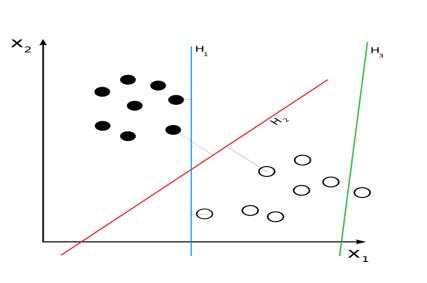
\includegraphics[height=3in,width=3in]
{svm.jpg}  
\caption{Support Vector Machine}
\end{center}
\end{figure} 

\subsubsection{Support and Error}
   \begin{itemize}
   \item \textbf{Support:} Support refers to the number of correctly classified samples by the rule, divided by the number of correctly classified samples by the NN.
   \item	\textbf{Error:} Error refers to number of wrong classified samples by the rule, divided by number of samples in the rule.
   \end{itemize}

\subsection{Software Requirements}
\subsubsection{Functional Requirement}
Creating a User Interface for demonstrating diabetes patient’s classification in positive or negative test with justification. 
   \begin{itemize}
   \item The process involves in step one of module one is creating feed-forward neural network with input, hidden and output layer and training of it using appropriate training algorithm. Defining goal and hidden layers neurons for achieving good accuracy.
   \item In the second step pruning process applied on trained network to prune the unwanted and zeroed valued network connections with attributed values. 
   \item Second module involves use of decision tree algorithm for discrete rule generation form trained network .Support of each rule is validated using separate C module for rule refinement.
   \item Third module involves use of support vector machine for hyper plane generation for contentious attributes.
   \end{itemize}
\subsubsection{Non-Functional Requirement}
The project requires standard dataset of the Pima Indian diabetes patients.
   \begin{itemize}
   \item\textbf{Maintainability:} All modules interfaces must be clearly define to change for the future technologies. Through thoughtful and effective software engineering, all steps of the software development process will be well documented to ensure maintainability of the product throughout its life time. All development will be provided with good documentation.
   \item \textbf{Performance:} The response time, utilization and throughput behavior of the system. Care is taken so as to ensure a system with comparatively high performance.
   \item \textbf{Usability:} The ease of use and training the end users of the system is usability. System should have qualities like- learning ability, efficiency, affect, control. The main aim of the project is to reduce server failure and gets high performance of server and reduces the rework of the programmer.
   \item \textbf{Modifiability:} The ease with which a software system can accommodate changes to its software is modifiability. Our project is easily adaptable for changes that is useful for the application to withstand the needs of the users.
   \item \textbf{Portability:} The ability of the system to run under different computing environments. The environment types can be either hardware or software, but is usually a combination of two.
   \item \textbf{Reusability:} The extent to which existing application can be reused in new application. Our application can be reused a number of times without any technical difficulties.
   \item \textbf{Security:} The factors that protect the software from accidental or malicious access, use, modification, destruction, or disclosure. Security can be ensured as the project involves authenticating the users.
   \end{itemize}

\subsection{Methodologies/Techniques to be used for knowledge extraction}
The Multilayer Perceptrons are used in this study make use of biases, sigmoid         activation functions and one hidden layer with a variable number of nodes.
   \begin{itemize}
   \item Back propagation algorithm for training ANN (Gradient steepest descent algorithm)
   \item C 4.5 algorithm
   \item MATLAB (MATrix LABoratory) Neural Network Toolbox 4.0 from Math Works Corp. is applied to perform the training exercises. 
   \item Neural network packages: Neurodimensions’ Neurosolutions v3.0 and Thinkspro v1.05 by Logical Designs Consulting.
   \item Support  Vector Machine algorithm
   \item Credit Approval dataset from UCI machine repository.
   \end{itemize}

\subsection{Features}
   \begin{itemize}
  \item Easy user interface 
  \item Online database creation for new and unknown data samples.
  \item Clear justification of the test report using rule extracted from the network..
  \item High accuracy on standard dataset.
  \item Can handle unknown and null values samples.
  \item Performance is good as advances training algorithm is used.
   \end{itemize}

\newpage
\section{PROJECT PLANNING AND MANAGEMENT}
\subsection{Project Process Management}
The V-model represents a software development process (also applicable to hardware development) which may be considered an extension of the waterfall model. Instead of moving down in a linear way, the process steps are bent upwards after the coding phase, to form the typical V shape. The V-Model demonstrates the relationships between each phase of the development life cycle and its associated phase of testing. The horizontal and vertical axes represents time or project completeness (left-to-right) and level of abstraction (coarsest-grain abstraction uppermost), respectively.

\begin{figure}[h]
\begin{center}
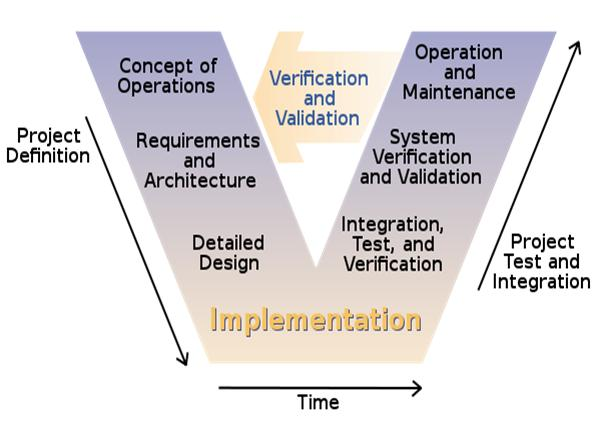
\includegraphics[height=3in,width=4in]
{vcycle.jpg}  
\caption{V Life Cycle Model}
\end{center}
\end{figure}

\subsection{Verification Phases}
\subsubsection{Requirements analysis}
\begin{sloppypar}
In the Requirements analysis phase, the first step in the verification process, the requirements of the proposed system are collected by analyzing the needs of the user(s). This phase is concerned with establishing what the ideal system has to perform. However it does not determine how the software will be designed or built. Usually, the users are interviewed and a document called the user requirements document is generated.
\end{sloppypar}
\begin{sloppypar}
The user requirements document will typically describe the system’s functional, interface, performance, data, security, etc requirements as expected by the user. It is used by business analysts to communicate their understanding of the system to the users. The users carefully review this document as this document would serve as the guideline for the system designers in the system design phase. The user acceptance tests are designed in this phase. See also Functional requirements. this is parallel processing.\end{sloppypar}
\begin{sloppypar}
There are different methods for gathering requirements of both soft and hard methodologies including; interviews, questionnaires, document analysis, observation, throw-away prototypes, use cases and status and dynamic views with users.\end{sloppypar}

\subsubsection{System Design}
\begin{sloppypar}
Systems design is the phase where system engineers analyze and understand the business of the proposed system by studying the user requirements document. They figure out possibilities and techniques by which the user requirements can be implemented. If any of the requirements are not feasible, the user is informed of the issue. A resolution is found and the user requirement document is edited accordingly.\end{sloppypar}
\begin{sloppypar}
The software specification document which serves as a blueprint for the development phase is generated. This document contains the general system organization, menu structures, data structures etc. It may also hold example business scenarios, sample windows, reports for the better understanding. Other technical documentation like entity diagrams, data dictionary will also be produced in this phase. The documents for system testing are prepared in this phase.
\end{sloppypar}

\subsubsection{Architecture Design}
   The phase of the design of computer architecture and software architecture can also be referred to as high-level design. The baseline in selecting the architecture is that it should realize all which typically consists of the list of modules, brief functionality of each module, their interface relationships, dependencies, database tables, architecture diagrams, technology details etc. The integration testing design is carried out in the particular phase.

\subsubsection{Module Design}
The module design phase can also be referred to as low-level design. The designed system is broken up into smaller units or modules and each of them is explained so that the programmer can start coding directly. The low level design document or program specifications will contain a detailed functional logic of the module, in pseudocode:
   \begin{itemize}
   \item Database tables, with all elements, including their type and size.
   \item All interface details with complete API references.
   \item All dependency issues.
   \item 	Error message listings.
   \item Complete input and outputs for a module.
   \item The unit test design is developed in this stage.
   \end{itemize}

\subsubsection{Module Design}
   \begin{itemize}
   \item Unit Testing
   \item Integration Testing
   \item System Testing
   \item User Acceptance Testing
   \item Acceptance testing helps
   \end{itemize}

\subsubsection{Feasibility Study}
Literature survey basically focuses on answer to, how well our project does satisfy the four dimensions:
   \begin{enumerate}
   \item Technology Feasibility
   \item Economic Feasibility
   \item Time Feasibility
   \item Resources Feasibility
   \end{enumerate}
Answer to these questions could be very easy for projects in established area where we get lots of time and resources to use and as the risks increases the feasibility study would result Negative.
As far our current project is concerned we have carried out the initial risk architecture and design so, that the above questions would be accurately answered.
  \begin{enumerate}
   \item \textbf{Technology Feasibility:}\\The project needs knowledge of MATLAB,Data Mining,Neural Network,Decision Tree Algorithm,Weka tool. As we have enough resources of both the technologies, we are capable to satisfy the technological needs of the project completely as well we do not need additional software or hardware to develop application.
   \item \textbf{Financial Feasibility:}\\As this project does not need any special hardware or licensed software and as the developer are going through their training, financial feasibility is not the problem for the organization. Moreover the organization already has enough infrastructures to support their application well so there is no need for any finance. 
   \item \textbf{Time Feasibility:}\\The project has to be completed by 10 months approx., as we have gathered requirements and analyzed them properly; it seems that project will be completed in time span provided. Therefore the project is feasible in time. 
   \item \textbf{Resource Feasibility:}\\The hardware and software components and human resources availability is sufficient enough to engineer the project. Hence the software is feasible considering resources.
   \end{enumerate}

\subsection{Cost and Effort Estimation}
\begin{itemize}
\item \textbf{Total Resources Estimation :}\\
   We know that the cost of developing software, up until the point it is accepted, is only a fraction of the total cost of the system over the typical life cycle of the product. However for the purpose of this study we will exclude to maintenance costs, and will speak only of the development costs up until acceptance.
\item \textbf{Functions:}\\
Cost estimation based on expected functionality of the system was first purposed by Albrecht in 1979, and has since been researched by several people. This Cost estimation realizes on function points and requires the identification of all occurrences of five unique functions types :External  Input ,External  Output  ,Logical internal files ,External Interfaces and queries .The sum of all occurrences is called RAW-FUNCTION-COUNTS (FC).This value must be modifies by the weighted rating of complexity factors ,giving a Technical Complexity Factor (TCF).The function points are equivalent to FC*TCF  for any given project. 
   \begin{itemize}
   \item Estimation of Hardware
           \begin{itemize}
           \item Minimum Requirement for Development
            \item Pentium 4 Processor
            \item 1 GB Of RAM
            \item 80 GB Hard Disk Space
            \end{itemize}
   \item Minimum Requirement for Execution
            \begin{itemize}
            \item Pentium 4 Processor
            \item 1 GB Of RAM
            \item 80 GB Hard Disk Space on server
           \end{itemize}
   \item Estimation Of  Software
            \begin{itemize}
            \item Software Resources
            \item MATLAB 7 or Higher version
            \item 	WEKA
            \end{itemize}
  \end{itemize}
\end{itemize}

 \subsection{Risk analysis and Management}
\begin{sloppypar}
Risk management is the identification, assessment, and prioritization of risks (defined in ISO 31000 as the effect of uncertainty on objectives, whether positive or negative) followed by coordinated and economical application of resources to minimize, monitor, and control the probability and/or impact of unfortunate events or to maximize the realization of opportunities. \end{sloppypar}
\begin{sloppypar}Risks can come from uncertainty in financial markets, project failures (at any phase in design, development, production, or sustainment life-cycles), legal liabilities, credit risk, accidents, natural causes and disasters as well as deliberate attack from an adversary, or events of uncertain or unpredictable root-cause.
\end{sloppypar}
\begin{sloppypar}
The strategies to manage risk typically include transferring the risk to another party, avoiding the risk, reducing the negative effect or probability of the risk, or even accepting some or all of the potential or actual consequences of a particular risk.
Risk management also faces difficulties in allocating resources. This is the idea of opportunity cost. Resources spent on risk management could have been spent on more profitable activities. Again, ideal risk management minimizes spending (or manpower or other resources) and also minimizes the negative effects of risks.
\end{sloppypar}

\subsubsection{Method}
For the most part, these methods consist of the following elements, performed, more or less, in the following order.
            \begin{itemize}
            \item Identify, characterize, and assess threats.
            \item Assess the vulnerability of critical assets to specific threats.
            \item Determine the risk (i.e. the expected likelihood and consequences of specific types of attacks on specific assets).
            \item Identify ways to reduce those risks.
            \item Prioritize risk reduction measures based on a strategy.
            \end{itemize}


\subsubsection{Risk management activities as applied to project management}
In project management, risk management includes the following activities:
            \begin{itemize}
            \item Planning how risk will be managed in the particular project. Plans should include risk management tasks, responsibilities, activities and budget.
            \item Assigning a risk officer - a team member other than a project manager who is responsible for foreseeing potential project problems. Typical characteristic of risk officer is a healthy skepticism.
            \item Maintaining live project risk database. Each risk should have the following attributes: opening date, title, short description, probability and importance. Optionally a risk may have an assigned person responsible for its resolution and a date by which the risk must be resolved.
            \item Creating anonymous risk reporting channel. Each team member should have the possibility to report risks that he/she foresees in the project.
            \item Preparing mitigation plans for risks that are chosen to be mitigated. The purpose of the mitigation plan is to describe how this particular risk will be handled – what, when, by who and how will it be done to avoid it or minimize consequences if it becomes a liability.
            \item Summarizing planned and faced risks, effectiveness of mitigation activities, and effort spent for the risk management.
            \end{itemize}

\subsubsection{Project Scheduling (timeline chart) }
\begin{table}[hbp]
 \begin{center}
    \begin{tabular}{ | l | p{5cm} | p{5cm} | l |}
    \hline
     Index  &	State	 & Tasks &	Time  \\ \hline
    1	& Requirement Gathering	& Requirements understanding, Use case design, functional requirements &	7 weeks\\ \hline
2	& Analysis  &	Design or select Architecture, framework Development, use case realization,Data Set preprocessing	& 7 weeks\\ \hline
3	& Design &	Develop Design model, MATLAB Network model designing,System Desingning &	11 weeks\\ \hline
4 	& Implementation	& Environmen setup, production rollout	  & 5 weeks\\ \hline
5	& Testing	& Goal matching,Fact table analysis,Accuracy mapping,Rule refinement	&   4 weeks\\ \hline
6	&  Deployment &	Integration of modules and deployment of application	 &  2 Week\\ \hline

    \hline
    \end{tabular}
   \caption{Plan of Execution}
\end{center}
\end{table} 

\textbf{Gantt chart:}\\
\begin{figure}[h!]
\begin{center}
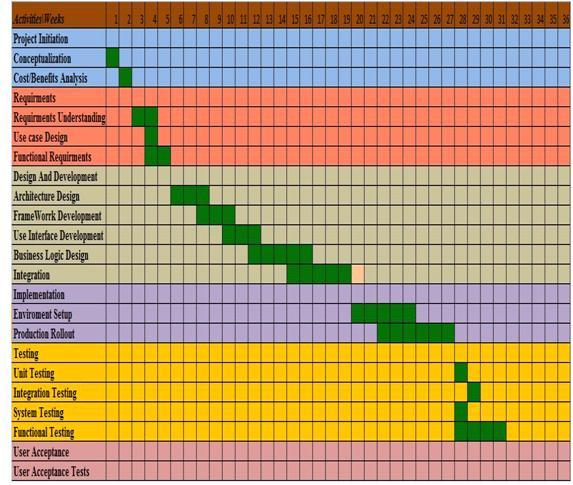
\includegraphics[height=3in,width=4in]
{gantt.jpg}  
\caption{Gantt chart}
\end{center}
\end{figure}  

\textbf{Timeline chart:}\\
 \begin{figure}[h!]
\begin{center}
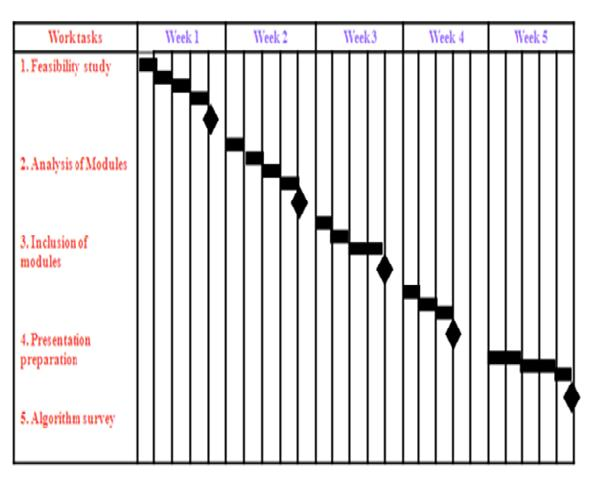
\includegraphics[height=3in,width=4in]
{timeline.jpg}  
\caption{Timeline chart}
\end{center}
\end{figure}

\newpage
\section{ANALYSIS AND DESIGN}
Design modeling uses a combination of text and diagrammatic forms to depict the requirements for data, function and behavior in a way that s relatively easy to understand and more importantly straightforward to review for correctness, completeness and consistency.
\begin{sloppypar}
The unified modeling language (uml) is a graphical language for visualization, specifying, constructing and documenting the artifacts of a software intensive system. The uml gives a standard way to write systems blue prints, covering conceptual things, such as business processes and system functions, as well as concrete things, such as classes written in a specific programming language, database schemas and reusable software components.\end{sloppypar}
Here we have included the following uml diagrams:
\subsection{Use Case Diagram}
A use case diagram is a type of behavioral diagram defined by the Unified Modeling
Language (UML) and created from a Use-case analysis. Its purpose is to present a graphical
overview of the functionality provided by a system in terms of actors, their goals (represented as use cases), and any dependencies between those use cases. The main purpose of a use case
diagram is to show what system functions are performed for which actors. Roles of the actors in
the system can be depicted.\\

\begin{figure}[h!]
\begin{center}
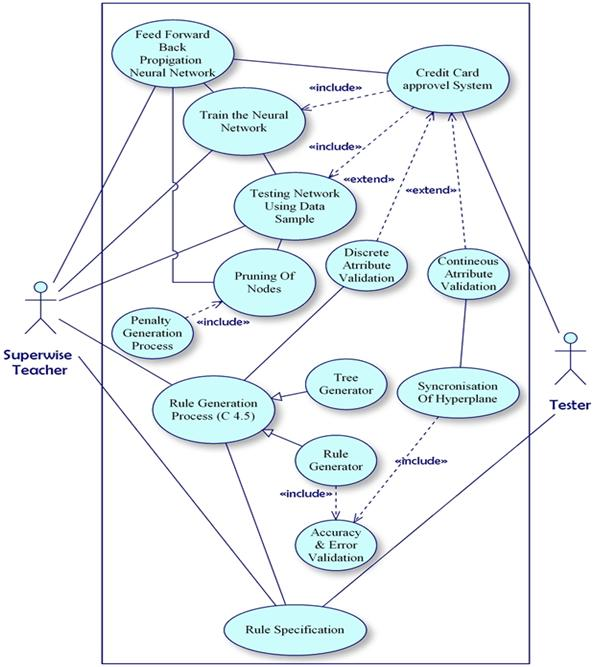
\includegraphics[height=4in,width=2.5in]
{UseCaseForReport.jpg} 
\caption{Use cases}
\end{center}
\end{figure}
\newpage
\subsection{Activity diagram}
An activity diagram is a diagram that shows activities and actions to describe workflows. In the Unified Modeling Language an activity diagram represents the business and operational step-by-step workflows of components in a system.\\ An activity diagram shows the overall flow of control.Activity diagrams are graphical representations of workflows of stepwise activities and actions with support for choice, iteration and concurrency. In the Unified Modeling Language, activity diagrams can be used to describe the business and operational step-by-step workflows of components in a system. An activity diagram shows the overall flow of control.
\begin{figure}[h!]
\begin{center}
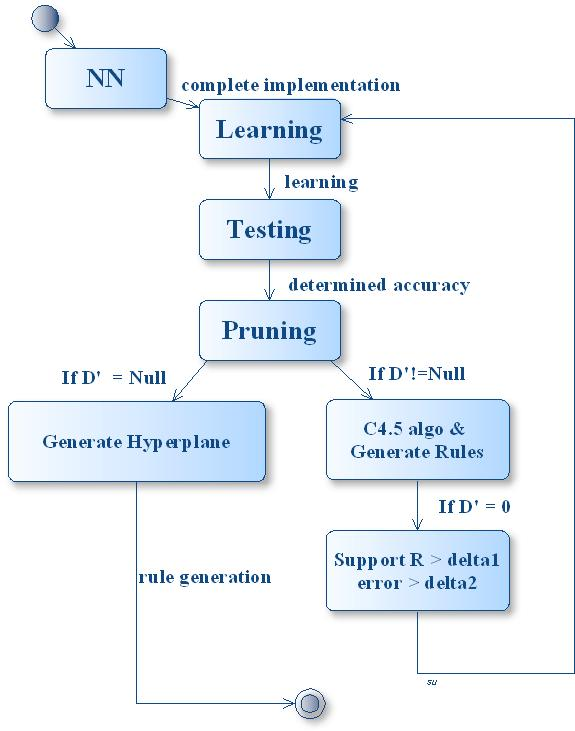
\includegraphics[height=5in,width=4in]
{state.jpg} 
\caption{Activity diagram}
\end{center}
\end{figure}

\newpage
\section{IMPLEMENTATION AND USER INTERFACES}
\subsection{Network Architecture}
The first step in training a feedforward network is to create the network object. The function newff creates a feedforward network. It requires four inputs and returns the network object.
\begin{figure}[h!]
\begin{center}
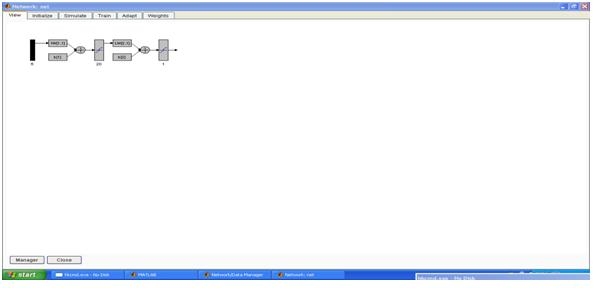
\includegraphics[height=3.5in,width=5.5in]
{NNArchi.jpg} 
\caption{ANN Architecture in MATLAB}
\end{center}
\end{figure}

\subsection{Network setup}
Network training involves numbers of attributes those are essential to achieve higher accuracy and optimal network.
\begin{itemize}
\item \textbf{Network learning rate:}            0.1
\item \textbf{Numbers of epoch:}                   1, 83525
\item \textbf{Network mean square error:}   0.1
\item \textbf{Goal achieved:}                           0.099999
\end{itemize}

\newpage
\subsection{Training of Neural network}
The training process requires a set of examples of proper network behavior - network inputs p and target outputs t. During training the weights and biases of the network are iteratively adjusted to minimize the network performance function net.performFcn.
\begin{figure}[h!]
\begin{center}
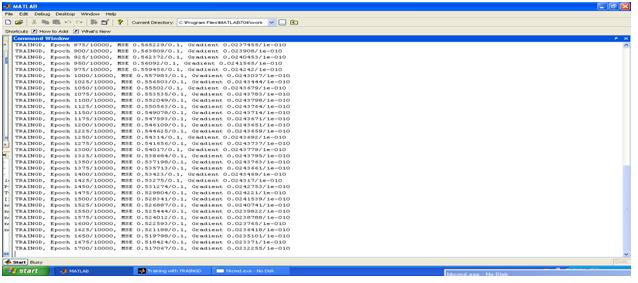
\includegraphics[height=3in,width=5in]
{NNTrain.jpg} 
\caption{ANN Training Process in MATLAB}
\end{center}
\end{figure}

\subsection{Training graph}
The result of training is shown in the following figure.
\begin{figure}[h!]
\begin{center}
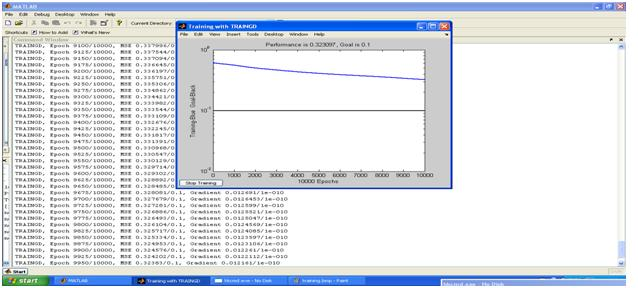
\includegraphics[height=3in,width=5in]
{NNTraing.jpg} 
\caption{ANN Training Graph in MATLAB}
\end{center}
\end{figure}


\subsection{Input \& Target Co-relation Graph}
Graph showing deviation between target and actual output.
\begin{figure}[h!]
\begin{center}
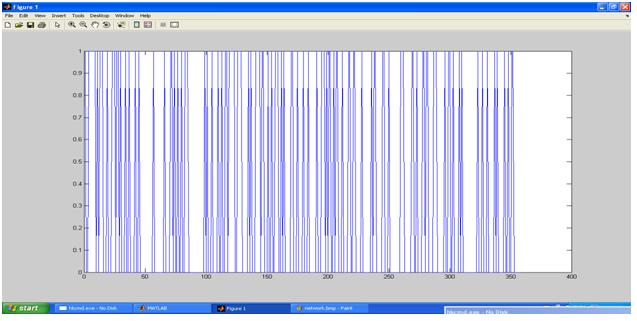
\includegraphics[height=3.5in,width=5in]
{NNDev.jpg} 
\caption{Deviation Graph in MATLAB}
\end{center}
\end{figure}


\subsection{Weka Decision tree Statistics }
Statesticis information generated by Weka on dataset using C4.5 algorithm.
\begin{figure}[h!]
\begin{center}
\includegraphics[height=3in,width=5in]
{Wekatree.jpg} 
\caption{Weka Decision tree Statistics}
\end{center}
\end{figure}



\subsection{Decision tree generated by Weka tool}
\begin{figure}[h!]
\begin{center}
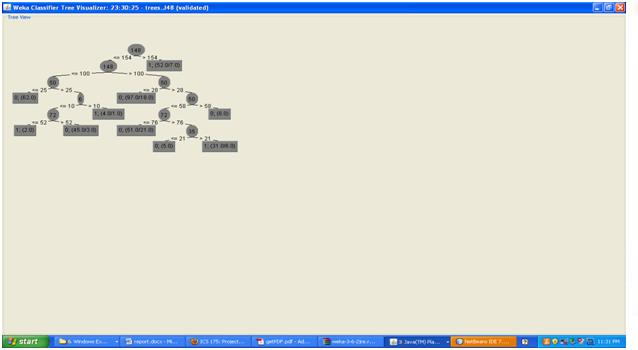
\includegraphics[height=2in,width=5in]
{WekaDecTree.jpg} 
\caption{Decision tree generated by Weka tool}
\end{center}
\end{figure}

\subsection{GUI of the System}
GUI tool for classifying user in positive or negative test with justification of NN output.
\begin{figure}[h!]
\begin{center}

\includegraphics[height=5in,width=5in]
{GUI.jpg} 
\caption{Graphical User Interface}
\end{center}
\end{figure}

\subsection{Code}
\subsubsection{Main Classification module with GUI}
\begin{itemize}
\item \textbf{index.jsp}
\begin{verbatim}
<!DOCTYPE html PUBLIC "-//W3C//DTD XHTML 1.0 Transitional//EN" "http://www.w3.org/TR/xhtml1/DTD/xhtml1-transitional.dtd">
<html xmlns="http://www.w3.org/1999/xhtml">
<head>
<meta http-equiv="Content-Type" content="text/html; charset=UTF-8" />
<title>Page - Diabetis Prediction Model</title>
<link rel="stylesheet" href="styles/style.css" type="text/css" media="screen" />
</head>
<body>

<div id="wrapper">
	<div id="header">
		<h1>Diabetis Prediction Model</h1>

		<div id="nav">
			<ul>
				<li><a href="index.jsp" id="nav1">Home</a></li>
				<li><a href="page.jsp" id="nav3">Neuro-Lab</a></li>
				<li><a href="about.jsp" id="nav4">About</a></li>
				<li><a href="contact.jsp" id="nav5">Contact</a></li>
			</ul>

		</div>
		<div class="clear"></div>
	</div>
	
	<div id="middlebar-small">
		<h2>Neuro Lab</h2>
	</div>
	
	<div id="body">	
		<div id="body-inner">			
			<div id="sidebar">

			    <h3 class="icon-feature">Authorised domain For Doctors.</h3>
				<hr></br></br>
				<p>Your valuable & Authorise feedback about Dibetes prediction will lead us to
                   improve the overall model.</br>
				   It will help us to</br>
                </p>   	
	            <ul>
					<li>To improve Regional Accuracy.</li>

					<li>To Normliase our Dataset.</a></li>
					<li>To Collect more Dataset on Dibetic Patients.</li>
				</ul>	
                </br>				
                <form id="form2" name="form2" method="post" action="SQLops_main.jsp">
				<ul class="Dform">
					<li><label for="Select Name">Name</label><font>:</font>&nbsp 
					  <select name="Uname">

                      <option value="Dr.A">Dr. A</option>
                      <option value="Dr.B">Dr. B</option>
                      <option value="Dr.C">Dr. C</option>
                      <option value="Dr.D">Dr. D</option>
                      </select> 
					</li>
					<li><label for="password">password</label><font>:</font>&nbsp

					<input name="password" type="password" /></li>
					<li><label for="Select Name">Outcome</label><font>:</font>&nbsp 
					  <select name="selectResult">
                      <option value="1">Right Prediction</option>
                      <option value="0">Wrong Prediction</option>
                      </select> 
					</li>
					</br>	
					<li><center><input type="submit" value="Send" class="button" /></center>

					</ul>
				    <hr>	
				</form>  
				</br><center><h3>Success!!</h3></center>
			</div>
			<div id="main-content">
				<form id="form1" name="form1" method="post" action="rules.jsp" >
				<h1>Check Out for Following symptoms</h1>
				</br><hr></br>

				<ul class="form">
					<li><label>1. Number of times pregnant</label><B>:</B>&nbsp <input name="ntp" type="text" value="3"/>&nbsp <font>*(0-17)</font></li>
					<li><label>2. Plasma glucose concentration</label><B>:</B>&nbsp <input name="pgc" type="text" value="66" />&nbsp <font>*(57-197)</font></li>
					<li><label>3. Diastolic blood pressure (mm Hg)</label><B>:</B>&nbsp <input name="dbp" type="text" value="45" />&nbsp <font>*(30-110)</font></li>

					<li><label>4. Triceps skin fold thickness (mm)</label><B>:</B>&nbsp <input name="tsft" type="text" value="39" />&nbsp <font>*(7-63)</font></li>
					<li><label>5. 2-Hour serum insulin (mu U/ml)</label><B>:</B>&nbsp <input name="si" type="text" value="145" />&nbsp <font>*(0-846)</font></li>
					<li><label>6. Body mass index</label><B>:</B>&nbsp <input name="bmi" type="text" value="43.8" />&nbsp <font>*(0-67.1)&nbsp </font></li>

					<li><label>7. Diabetes pedigree function</label><B>:</B>&nbsp <input name="dpf" type="text" value="0.45" />&nbsp <font>*(0.078-2.42)</font></li>
					<li><label>8. Age</label><B>:</B>&nbsp <input name="age" type="text" value="34" />&nbsp <font>*(21-81)</font></li>
					</br></br>
				</ul>

     			 <center><input type="submit" value="Submit Query" class="button" /></center>
				</form> 
				</br>
				<center><h2>Tested *Negative for Diabetes</h2></center>				
				</br></br>
				<form id="form1" name="form2" method="post" action="justfy.jsp" >
				<center><input type="submit" value="Justify Your Prediction" class="button" /><center>
                </br>
				<ul>

				<li><b>Plasma glucose concentration is Less than 155.</b></li><li><b>Age of the pantient is Greater than 25 Years.</b></li><li><b>Pantient is pregnant less than 11 times.</b></li><li><b>Diastolic blood pressure is less than 53 (mm hg)</b></li>
				</ul>
				</form>
			</div>
		</div>
	</div>

	<div id="footer">
		<div id="footer-right">
			<a href="index.jsp">Home</a> |
			<a href="page.jsp">Neuro-Lab</a> |
			<a href="about.jsp">About</a> |
			<a href="contact.jsp">Contact</a>
		</div>

		Copyright &copy; 2012 Neural Network Group 
	</div>
</div>

</body>
</html>
\end{verbatim}
\end{itemize}

\subsubsection{Module for feed-forward NN}
\begin{verbatim}
function net = newff(pr,s,tf,btf,blf,pf)
if nargin < 2
net = newnet('newff');
return
end

% Defaults
if nargin < 4, btf = 'trainlm'; end
if nargin < 5, blf = 'learngdm'; end
if nargin < 6, pf = 'mse'; end

% Error checking
if (~isa(pr,'double')) | ~isreal(pr) | (size(pr,2) ~= 2)
error('Input ranges is not a two column matrix.')
end
if any(pr(:,1) > pr(:,2))
error('Input ranges has values in the second column larger in the values in the same row of the first column.')
end
if isa(s,'cell')
if (size(s,1) ~= 1)
error('Layer sizes is not a row vector of positive integers.')
end
for i=1:length(s)
si = s{i};
if ~isa(si,'double') | ~isreal(si) | any(size(si) ~= 1) | any(si<1) | any(round(si) ~= si)
error('Layer sizes is not a row vector of positive integers.')
end
end
s = cell2mat(s);
end
if (~isa(s,'double')) | ~isreal(s) | (size(s,1) ~= 1) | any(s<1) | any(round(s) ~= s)
error('Layer sizes is not a row vector of positive integers.')
end

% More defaults
Nl = length(s);
if nargin < 3, tf = {'tansig'}; tf = [tf(ones(1,Nl))]; end

% Architecture
net = network(1,Nl);
net.biasConnect = ones(Nl,1);
net.inputConnect(1,1) = 1;
[j,i] = meshgrid(1:Nl,1:Nl);
net.layerConnect = (j == (i-1));
net.outputConnect(Nl) = 1;
net.targetConnect(Nl) = 1;

% Simulation
net.inputs{1}.range = pr;
for i=1:Nl
net.layers{i}.size = s(i);
net.layers{i}.transferFcn = tf{i};
end

% Performance
net.performFcn = pf;

% Adaption
net.adaptfcn = 'trains';
net.inputWeights{1,1}.learnFcn = blf;
for i=1:Nl
net.biases{i}.learnFcn = blf;
net.layerWeights{i,:}.learnFcn = blf;
end

% Training
net.trainfcn = btf;

% Initialization
net.initFcn = 'initlay';
for i=1:Nl
net.layers{i}.initFcn = 'initnw';
end
net = init(net);

\end{verbatim}

\subsubsection{NN training module}
\begin{verbatim}
function [net,tr,Y,E,Pf,Af]=train(net,P,T,Pi,Ai,VV,TV)
if nargin < 2
error('Not enough input arguments.');
end
if ~isa(net,'network')
error('First argument is not a network.');
end
if net.hint.zeroDelay
error('Network contains a zero-delay loop.')
end
switch nargin
case 2
[err,P,T,Pi,Ai,Q,TS,matrixForm] = trainargs(net,P);
VV = [];
TV = [];
case 3
[err,P,T,Pi,Ai,Q,TS,matrixForm] = trainargs(net,P,T);
VV = [];
TV = [];
case 4
[err,P,T,Pi,Ai,Q,TS,matrixForm] = trainargs(net,P,T,Pi);
VV = [];
TV = [];
case 5
[err,P,T,Pi,Ai,Q,TS,matrixForm] = trainargs(net,P,T,Pi,Ai);
VV = [];
TV = [];
case 6
[err,P,T,Pi,Ai,Q,TS,matrixForm] = trainargs(net,P,T,Pi,Ai);
if isempty(VV)
VV = [];
else
if ~hasfield(VV,'P'), error('VV.P must be defined or VV must be [].'), end
if ~hasfield(VV,'T'), VV.T = []; end
if ~hasfield(VV,'Pi'), VV.Pi = []; end
if ~hasfield(VV,'Ai'), VV.Ai = []; end
[err,VV.P,VV.T,VV.Pi,VV.Ai,VV.Q,VV.TS,matrixForm] = ...
trainargs(net,VV.P,VV.T,VV.Pi,VV.Ai);
if length(err)
disp('??? Error with validation vectors using ==> train')
error(err)
end
end
TV = [];
case 7
[err,P,T,Pi,Ai,Q,TS,matrixForm] = trainargs(net,P,T,Pi,Ai);
if isempty(VV)
VV = [];
else
if ~hasfield(VV,'P'), error('VV.P must be defined or VV must be [].'), end
if ~hasfield(VV,'T'), VV.T = []; end
if ~hasfield(VV,'Pi'), VV.Pi = []; end
if ~hasfield(VV,'Ai'), VV.Ai = []; end
[err,VV.P,VV.T,VV.Pi,VV.Ai,VV.Q,VV.TS,matrixForm] = ...
trainargs(net,VV.P,VV.T,VV.Pi,VV.Ai);
if length(err)
disp('??? Error with validation vectors using ==> train')
error(err)
end
end
if isempty(TV)
TV = [];
else
if ~hasfield(TV,'P'), error('TV.P must be defined or TV must be [].'), end
if ~hasfield(TV,'T'), TV.T = []; end
if ~hasfield(TV,'Pi'), TV.Pi = []; end
if ~hasfield(TV,'Ai'), TV.Ai = []; end
[err,TV.P,TV.T,TV.Pi,TV.Ai,TV.Q,TV.TS,matrixForm] = ...
trainargs(net,TV.P,TV.T,TV.Pi,TV.Ai);
if length(err)
disp('??? Error with test vectors using ==> train')
error(err)
end
end
end
if length(err), error(err), end

% TRAIN NETWORK
% -------------
 
% Training function
trainFcn = net.trainFcn;
if ~length(trainFcn)
error('Network "trainFcn" is undefined.')
end

% Delayed inputs, layer targets
Pc = [Pi P];
Pd = calcpd(net,TS,Q,Pc);
Tl = expandrows(T,net.hint.targetInd,net.numLayers);

% Validation and Test vectors
doValidation = ~isempty(VV);
doTest = ~isempty(TV);
if (doValidation)
VV.Pd = calcpd(net,VV.TS,VV.Q,[VV.Pi VV.P]);
VV.Tl = expandrows(VV.T,net.hint.targetInd,net.numLayers);
end
if (doTest)
TV.Pd = calcpd(net,TV.TS,TV.Q,[TV.Pi TV.P]);
TV.Tl = expandrows(TV.T,net.hint.targetInd,net.numLayers);
end

% Train network
net = struct(net);
flatten_time = (net.numLayerDelays == 0) & (TS > 1) & (~strcmp(trainFcn,'trains'));
if flatten_time
Pd = seq2con(Pd);
Tl = seq2con(Tl);
if (doValidation)
VV.Pd = seq2con(VV.Pd);
VV.Tl = seq2con(VV.Tl);
VV.Q = VV.Q*VV.TS;
VV.TS = 1;
end
if (doTest)
TV.Pd = seq2con(TV.Pd);
TV.Tl = seq2con(TV.Tl);
TV.Q = TV.Q*TV.TS;
TV.TS = 1;
end
[net,tr,Ac,El] = feval(trainFcn,net,Pd,Tl,Ai,Q*TS,1,VV,TV);
Ac = con2seq(Ac,TS);
El = con2seq(El,TS);
else
[net,tr,Ac,El] = feval(trainFcn,net,Pd,Tl,Ai,Q,TS,VV,TV);
end
net = class(net,'network');

% Network outputs, errors, final inputs
Y = Ac(net.hint.outputInd,net.numLayerDelays+[1:TS]);
E = El(net.hint.targetInd,:);
Pf = Pc(:,TS+[1:net.numInputDelays]);
Af = Ac(:,TS+[1:net.numLayerDelays]);

% FORMAT OUTPUT ARGUMENTS
% -----------------------

if (matrixForm)
Y = cell2mat(Y);
E = cell2mat(E);
Pf = cell2mat(Pf);
Af = cell2mat(Af);
end

% CLEAN UP TEMPORARY FILES
% ------------------------
nntempdir=fullfile(tempdir,'matlab_nnet');
if exist(nntempdir)
rmpath(nntempdir);
tf=dir(nntempdir);
for i=1:length(tf)
if (~tf(i).isdir)
delete(fullfile(nntempdir,tf(i).name));
end
end
rmdir(nntempdir)
end

% ============================================================
function [s2] = expandrows(s,ind,rows)

s2 = cell(rows,size(s,2));
s2(ind,:) = s;

% ============================================================
function [err,P,T,Pi,Ai,Q,TS,matrixForm] = trainargs(net,P,T,Pi,Ai);

% Check signals: all matrices or all cell arrays
% Change empty matrices/arrays to proper form
switch class(P)
case 'cell', matrixForm = 0; name = 'cell array'; default = {};
case {'double','logical'}, matrixForm = 1; name = 'matrix'; default = [];
otherwise, err = 'P must be a matrix or cell array.'; return
end
if (nargin < 3)
T = default;
elseif ((isa(T,'double')|isa(T,'logical')) ~= matrixForm)
if isempty(T)
T = default;
else
err = ['P is a ' name ', so T must be a ' name ' too.'];
return
end
end
if (nargin < 4)
Pi = default;
elseif ((isa(Pi,'double')|isa(Pi,'logical')) ~= matrixForm)
if isempty(Pi)
Pi = default;
else
err = ['P is a ' name ', so Pi must be a ' name ' too.'];
return
end
end
if (nargin < 5)
Ai = default;
elseif ((isa(Ai,'double')|isa(Ai,'logical')) ~= matrixForm)
if isempty(Ai)
Ai = default;
else
err = ['P is a ' name ', so Ai must be a ' name ' too.'];
return
end
end

% Check Matrices, Matrices -> Cell Arrays
if (matrixForm)
[R,Q] = size(P);
TS = 1;
[err,P] = formatp(net,P,Q); if length(err), return, end
[err,T] = formatt(net,T,Q,TS); if length(err), return, end
[err,Pi] = formatpi(net,Pi,Q); if length(err), return, end
[err,Ai] = formatai(net,Ai,Q); if length(err), return, end
  
% Check Cell Arrays
else
d  [R,TS] = size(P);
  [R1,Q] = size(P{1,1});
  [err] = checkp(net,P,Q,TS); if length(err), return, end
  [err,T] = checkt(net,T,Q,TS); if length(err), return, end
  [err,Pi] = checkpi(net,Pi,Q); if length(err), return, end
  [err,Ai] = checkai(net,Ai,Q); if length(err), return, end
end
\end{verbatim}

\section{TESTING}
\subsection{NN Result with 12 hidden nodes}
\begin{table}[hbp]
 \begin{center}
    \begin{tabular}{ | p{4cm} | p{4cm} | p{4cm} | p{3cm} |}
    \hline
     Training+validation & Correctly Classified & Wrong Classified	& \%Accuracy  \\ \hline
316  &	283 &  33 & 	89.55\% \\ \hline
Testing Samples & 	Correctly Classified	 &  Wrong Classified	&  \%Accuracy\\ \hline
216	&  162 &  	54	 &  75\%\\      \hline
       \end{tabular}
   \caption{Fact table with 12 hidden nodes}
\end{center}
\end{table} 

\subsection{NN Result with 20 hidden nodes}
\begin{table}[hbp]
 \begin{center}
    \begin{tabular}{ | p{4cm} | p{4cm} | p{4cm} | p{3cm} |}
    \hline
     Training+validation & Correctly Classified & Wrong Classified	& \%Accuracy  \\ \hline
366	& 357 &	9	& 97.54\% \\ \hline
Testing Samples & 	Correctly Classified	 &  Wrong Classified	&  \%Accuracy\\ \hline
166	& 121 & 45	 & 72.89\%\\  \hline
       \end{tabular}
   \caption{Fact table with 20 hidden nodes}
\end{center}
\end{table} 

\newpage
\subsection{Rules Table}
\begin{table}[hbp]
 \begin{center}
    \begin{tabular}{ | l | l | l | l | l | p{1cm}| }
    \hline
     Rule No. & No. of samples &	Correctly classified &	Wrong Classified &  \%Support & \%Error \\ \hline
R1	& 62	& 62	& 0	& 17.32	 & 0 \\ \hline
R2	& 2	& 2	& 0	& 0.56 &	0 \\ \hline
R3	& 45	 & 42	& 3	& 12.57 	& 6.67 \\ \hline
R4	& 4	& 3	& 1 & 1.12	& 25 \\ \hline
R5	& 97	& 79	& 18	& 27.09	 & 18.56 \\ \hline
R6	& 52	& 30	& 22	& 14.52	 & 42.31 \\ \hline
R7	& 5 &	5	& 0	& 1.4	& 0 \\ \hline
R8	& 31	& 25	& 6	& 8.66	& 19.35 \\ \hline
R9	& 8	& 8	& 0	& 2.23	& 0 \\ \hline
R10	& 52	& 45	& 7	& 14.52 	& 13.45 \\ \hline
\, & 358 &  301 & 57 &  \, & \,\\ \hline
       \end{tabular}
   \caption{Rules Table}
\end{center}
\end{table} 

\subsection{Rules generated using Discrete Attributes}
\begin{verbatim}
Rule R1: If D2<=154 and D2<=100 and D5<=25, then Predict Class 0.
Rule R2: If D2<=154 and D2<=100 and D5>25 and D1<=10 and D3<=52, then Predict  Class1.
Rule R3: If D2<=154 and D2<=100 and D5>25 and D1<=10 and D3>52, then Predict Class0.
Rule R4: If D2<=154 and D2<=100 and D5>25 and D1>10, then Predict Class 1.
Rule R5: If D2<=154 and D2>100 and D5<=28, then Predict Class0.
Rule R6: If D2<=154 and D2>100 and D5>28 and D5<=58 and D3<=76, then Predict Class0.
Rule R7: If D2<=154 and D2>100 and D5>28 and D5<=58 and D3>76 and D4<=21, then Predict Class0.
Rule R8: If D2<=154 and D2>100 and D5>28 and D5<=58 and D3>76 and D4>21, then Predict Class1.
Rule R9: If D2<=154 and D2>100  and D5>58, then Predict class0
Rule 10: If D2>154 then, Predict Class 1.
\end{verbatim}

\newpage
\section{APPLICATION}
\subsection{Business Applications}
The 1988 DARPA Neural Network Study [DARP88] lists various neural network applications, beginning in about 1984 with the adaptive channel equalizer. This device, which is an outstanding commercial success, is a single- neuron network used in long-distance telephone systems to stabilize voice signals. The DARPA report goes on to list other commercial applications, including a small word recognizer, a process monitor, a sonar classifier, and a risk analysis system. Neural networks have been applied in many other fields since the DARPA report was written. A list of some applications mentioned in the literature follows:
\subsection{Credit Card Activity Checking}
Neural networks are used to spot unusual credit card activity that might possibly be associated with loss of a credit card. 
\subsection{Financial}
Real estate appraisal, loan advisor, mortgage screening, corporate bond rating, credit-line use analysis, portfolio trading program, corporate financial analysis, currency price prediction. 
\subsection{Medical and Banking}
Breast cancer cell analysis, EEG and ECG analysis, prosthesis design, optimization of transplant times, hospital expense reduction, hospital quality improvement, emergency-room test advisement 
How can I tell which transactions are likely to be fraudulent.?
\subsection{FUTURE ENHANCEMENTS}
  \begin{itemize}
  \item Rule optimization using Genetic Algorithm.
  \item Extending RE-RX to multiple group classification problem.
  \item Base can be changed from C4.5 to C5.0.
  \item Replacing hyper plane by the technique to handle inseparability.
  \end{itemize}

\newpage
\section{CONCLUSTION}
We have developed a new NN rule extraction algorithm Re-RX that is capable of extracting classification rules from NNs trained using both discrete and continuous attributes.The novel characteristic of the algorithm lies in its hierarchical nature of considering discrete variables before continuous variables,in a recursive way. We have illustrated the working of the algorithm using three real-world data sets. More specifically,we have considered application scoring where classification models are built to distinguish good payers from defaulters based on the characteristics provided at the time of application.Two key requirements of application scoring models are performance and interpretability. Especially, the latter is becoming more and more important since financial regulators and law enforcement bodies require all risk management models of a financial institution to be validated. Using real-life application scoring data sets, we have demonstrated that Re-RX is able to extract accurate and interpretable classification rules.There is an obvious limitation to the applicability of the proposed algorithm, however. When the class labels of the data are best described as a nonlinear function of the continuous inputs,the extracted rules will not be able to preserve the accuracy of the NN. This is a consequence of the property of Re-RX which generates only linear classifiers involving the continuous attributes in order to improve the comprehensibility of the overall rule set. It is possible to preserve the accuracy, for example, by having an NN or other nonlinear classifiers, in place of the linear hyperplane. However, such rules would not be as comprehensible as Re-RX generated rules. The issue of accuracy versus complexity and comprehensibility of the rules generated from trained NNs certainly deserves further research.

\newpage
\appendix
\section{Recursive Neural Network Rule Extraction
for Data With Mixed Attributes [Re-Rx] Algorithm}
\rule{6.3in}{.02in}
 \\Algorithm \emph{Re-Rx(S,D,C)}\\
\rule{6.3in}{.02in}
\\Input  : A set of data samples S having discrete attributes
             D and continuous attributes C\\
Output: A set of classification rules.\\
\begin{enumerate}
\item Train and prune an NN using the data set S and all its attributes D and C.
\item Let $\acute{D}$ and $\acute{C}$ be the sets of discrete and continuous attributes still present in the network, respectively. Let $\acute{S}$ be the set of data samples that are correctly classified by the pruned network. 
\item If $\acute{D} = \emptyset$ , then generate a hyperplane to split the samples
in $\acute{S}$ according to the values of their continuous attributes $\acute{C}$
and stop.\\
 Otherwise, using only the discrete attributes $\acute{D}$, generate the
set of classification rules R for the data set $\acute{S}$.
\item For each rule ${R}_i$ generated:
If support ${R}_i > \delta_1$ and error  ${R}_i > \delta_2$ , then
\begin{itemize}
\item Let ${S}_i$ be the set of data samples that satisfy the condition
of rule ${R}_i$  and ${D}_i$  be the set of discrete attributes that do not
appear in rule condition of ${R}_i$ .
\item If $\acute{D} = \emptyset$ , then generate a hyperplane to split the samples
in ${S}_i$ according to the values of their continuous attributes ${C}_i$
and stop.
\item Otherwise, call \emph{Re-Rx(${S}_i$${D}_i$,${C}_i$)}
\end{itemize}
\end{enumerate}
\rule{6.3in}{.02in}


\newpage
\begin{thebibliography}{00}
\bibitem{1} Extracting rules for classification problems: AIS based approach By Humar Kahramanli , Novruz Allahverdi [Science direct : Expert Systems with Applications xxx (2009) article in press]
\bibitem{2} Recursive Neural Network Rule Extraction for Data with Mixed attributes By Rudy Setiono,Senior Member, IEEE, Bart Baesens, and Christophe Mues [IEEE Transaction on Neural Networks, Vol. 19 No. 2, February 2008 pp. 299-307]
\bibitem{3} Data Mining:Concepts and techniques By Han J. , Kamber, M. Y. and Lee S. C.(2001).. San Francisco, CA, USA: Morgan Kaufmann.
\bibitem{4} Using neural networks and data mining techniques for the financial distress prediction model. By Wei-Sen Chen , Yin-Kuan Du [Science direct :Expert Systems with Applications 36 (2009) 4075–4086]
\bibitem{5} Data classification with Multilayer perceptrons using a generalized error function By Luís M. Silva a, J. Marques de Sá a,b, Luís A. Alexandre [Science direct : Neural Networks 21 (2008) 1302-1310]
\bibitem{6} Design of a hybrid system for the diabetes and heart diseases By Humar Kahramanli , Novruz Allahverdi [Science direct : Expert Systems with Applications 35 (2008) 82-89.
\bibitem{7} Mining Classification rules for Liver Disorders By Humar Kahramanli , Novruz Allahverdi International Journal of Mathematics and Computers in Simulatin Issue1, Volume 3, 2009.
\bibitem{8} Evaluation of neural networks and data mining methods on a credit assessment task for class imbalance problem. By Yueh-Min Huanga, Chun-Min Hunga, Hewijin Christine Jiaub [Science direct: Nonlinear Analysis: RealWorld Applications 7 (2006) 720 – 747 ]
\bibitem{9} Humar Kahramanli , Novruz Allahverdi ,”A new method for composing classification rules: AR+OPTBP”, 5th International Advanced Technologies Symposium (IATS’09), May 13-15, 2009, Karabuk, Turkey. …
\bibitem{10} Evolution of neural networks for classification and regression By Miguel Rocha, Paulo Cortez, Jose Neves [Science direct : Neurocomputing 70 (2007) 2809–2816]
\bibitem{11} Generating rules with predicates, terms and variables from the pruned neural networks By Richi Nayak [Science direct : Neural Networks-Accepted in 6 Feb, 2009 Article in press]
\bibitem{12} Gallant, S. I. (1988). Connection expert systems. Communications of the ACM, 31(2), 152–169. 
\bibitem{13} R. Setiono and H. Liu, “Symbolic representation of neural networks,” IEEE Computer, vol. 29, no. 3, pp. 71–77, Mar. 1996.
\bibitem{14} R. Setiono, “Extracting rules from neural networks by pruning and hidden-unit splitting,” Neural Comput., vol. 9, no. 1, pp. 205–225, 1997.
\bibitem{15} A. Gupta, S. Park, and S. M. Lam, “Generalized analytic rule extraction for feedforward neural networks,” IEEE Trans. Knowl. Data Eng., vol. 11, no. 6, pp. 985–991, Nov./Dec. 1999.
\bibitem{16} T. A. Etchells and J. P. G. Lisboa, “Orthogonal search-based rule extraction (OSRE) for trained neural-networks: A  practical and efficient approach,” IEEE Trans. Neural Netw., vol. 17, no. 2, pp. 374–384, Mar. 2006.
\bibitem{17} M. Craven and J. Shavlik, “Extracting tree-structured representations of trained networks,” in Advances in Neural Information Processing Systems (NIPS). Cambridge, MA:MIT Press, 1996, vol. 8, pp. 24–30.
\bibitem{18} D. Nauck and R. Kruse, “Neuro-fuzzy methods in fuzzy rule generation,” in Fuzzy Sets in Approximate Reasoning and Information Systems. Norwell, MA: Kluwer , 1999, pp. 305–334.
\bibitem{19} J. M. Benitez, J. L. Castro, and I. Requena, “Are neural network black boxes?,” IEEE Trans. Neural Netw., vol. 8, no. 5, pp. 1156–1164, Sep. 1997.
\bibitem{20} H. Tsukimoto, “Extracting rules from trained neural networks,” IEEE Trans. Neural Netw., vol. 11, no. 2, pp. 377–389, Mar. 2000. 
\bibitem{21} I. A. Taha and J. Ghosh, “Symbolic interpretation of artificial neural networks,” IEEE Trans. Knowl. Data Eng., vol. 11, no. 3, pp. 448–463, May/Jun. 1999.
\bibitem{22} J. R. Rabunal, J. Dorado, A. Pazos, J. Periera, and D. Rivero, “A new approach to the extraction of ANN rules and to their generalization capacity through GP,” Neural Comput., vol. 16, no. 7, pp. 1483–1523, 2004. 
\end{thebibliography}
\end{document}
